\section{数据分析}

通过该AI辅助系统,本团队获得了大量高精度的实验数据。本节将详细分析这些数据,验证系统的有效性,并展示实验结果,验证相关物理规律。


\subsection{重力加速度测量的数据分析}


\subsubsection{重力加速度测量结果与对比}
本实验通过AI视觉跟踪技术测量单摆运动,实现了高精度重力加速度测定。实验使用摆长约0.35m,初始摆角5°,进行了5组重复测量,测量结果如下:

\begin{table}[H]
\centering
\caption{重力加速度多次测量结果汇总}
\begin{tabular}{@{}c c c c c c@{}}
\toprule
\textbf{实验编号} & \textbf{摆长(m)} & \textbf{测量方法} & \textbf{周期(s)} & \textbf{重力加速度(m/s$^2$)} & \textbf{相对误差(\%)} \\
\midrule
3501 & 0.3505 & FFT & 1.191 & 9.748 & 0.47 \\
3502 & 0.3501 & FFT & 1.189 & 9.781 & 0.12 \\
3503 & 0.3499 & FFT & 1.187 & 9.815 & 0.22 \\
3504 & 0.3495 & Peak & 1.189 & 9.783 & 0.11 \\
3505 & 0.3500 & Fit & 1.188 & 9.796 & 0.02 \\
\bottomrule
\end{tabular}
\label{tab:gravity_results}
\end{table}


根据李本苍等人的研究\textsuperscript{\cite{KJSJ201335139}},传统重力加速测量方法的误差如下:

\begin{table}[H]
\centering
\caption{传统重力加速度测量方法对比(重力加速度标准值9.78995 m/s$^2$)}
\begin{tabular*}{0.7\textwidth}{@{\extracolsep{\fill}} c c c @{}}
\toprule
\textbf{实验方法} & \textbf{测量结果 (m/s$^2$)} & \textbf{相对误差 (\%)} \\
\midrule
平衡法        & $g = 9.623$ & 1.71 \\
单摆法        & $g = 9.609$ & 1.85 \\
复摆法        & $g = 9.704$ & 0.87 \\
倾斜气垫导轨法 & $g = 9.712$ & 0.79 \\
\bottomrule
\end{tabular*}
\label{tab:traditional_methods}
\end{table}
其中平衡法又称阿特伍德机法,是英国剑桥大学数学家、物理学家乔治 •阿特伍德(George Atwood,1746 -1807)为了验证牛顿第二定律,在1784年发表了一篇题为《关于物体的直线运动和转动》的学术论文,提出的一种用于测量加速度及验证牛顿力学定律的机械装置\textsuperscript{\cite{JXWL201706004}},该装置对重力加速的测量精度有所提升,但仪器操作步骤复杂,且误差仍然较大。
\begin{figure}[H]
    \centering
    \subfigure[阿特伍德机示意图]{
        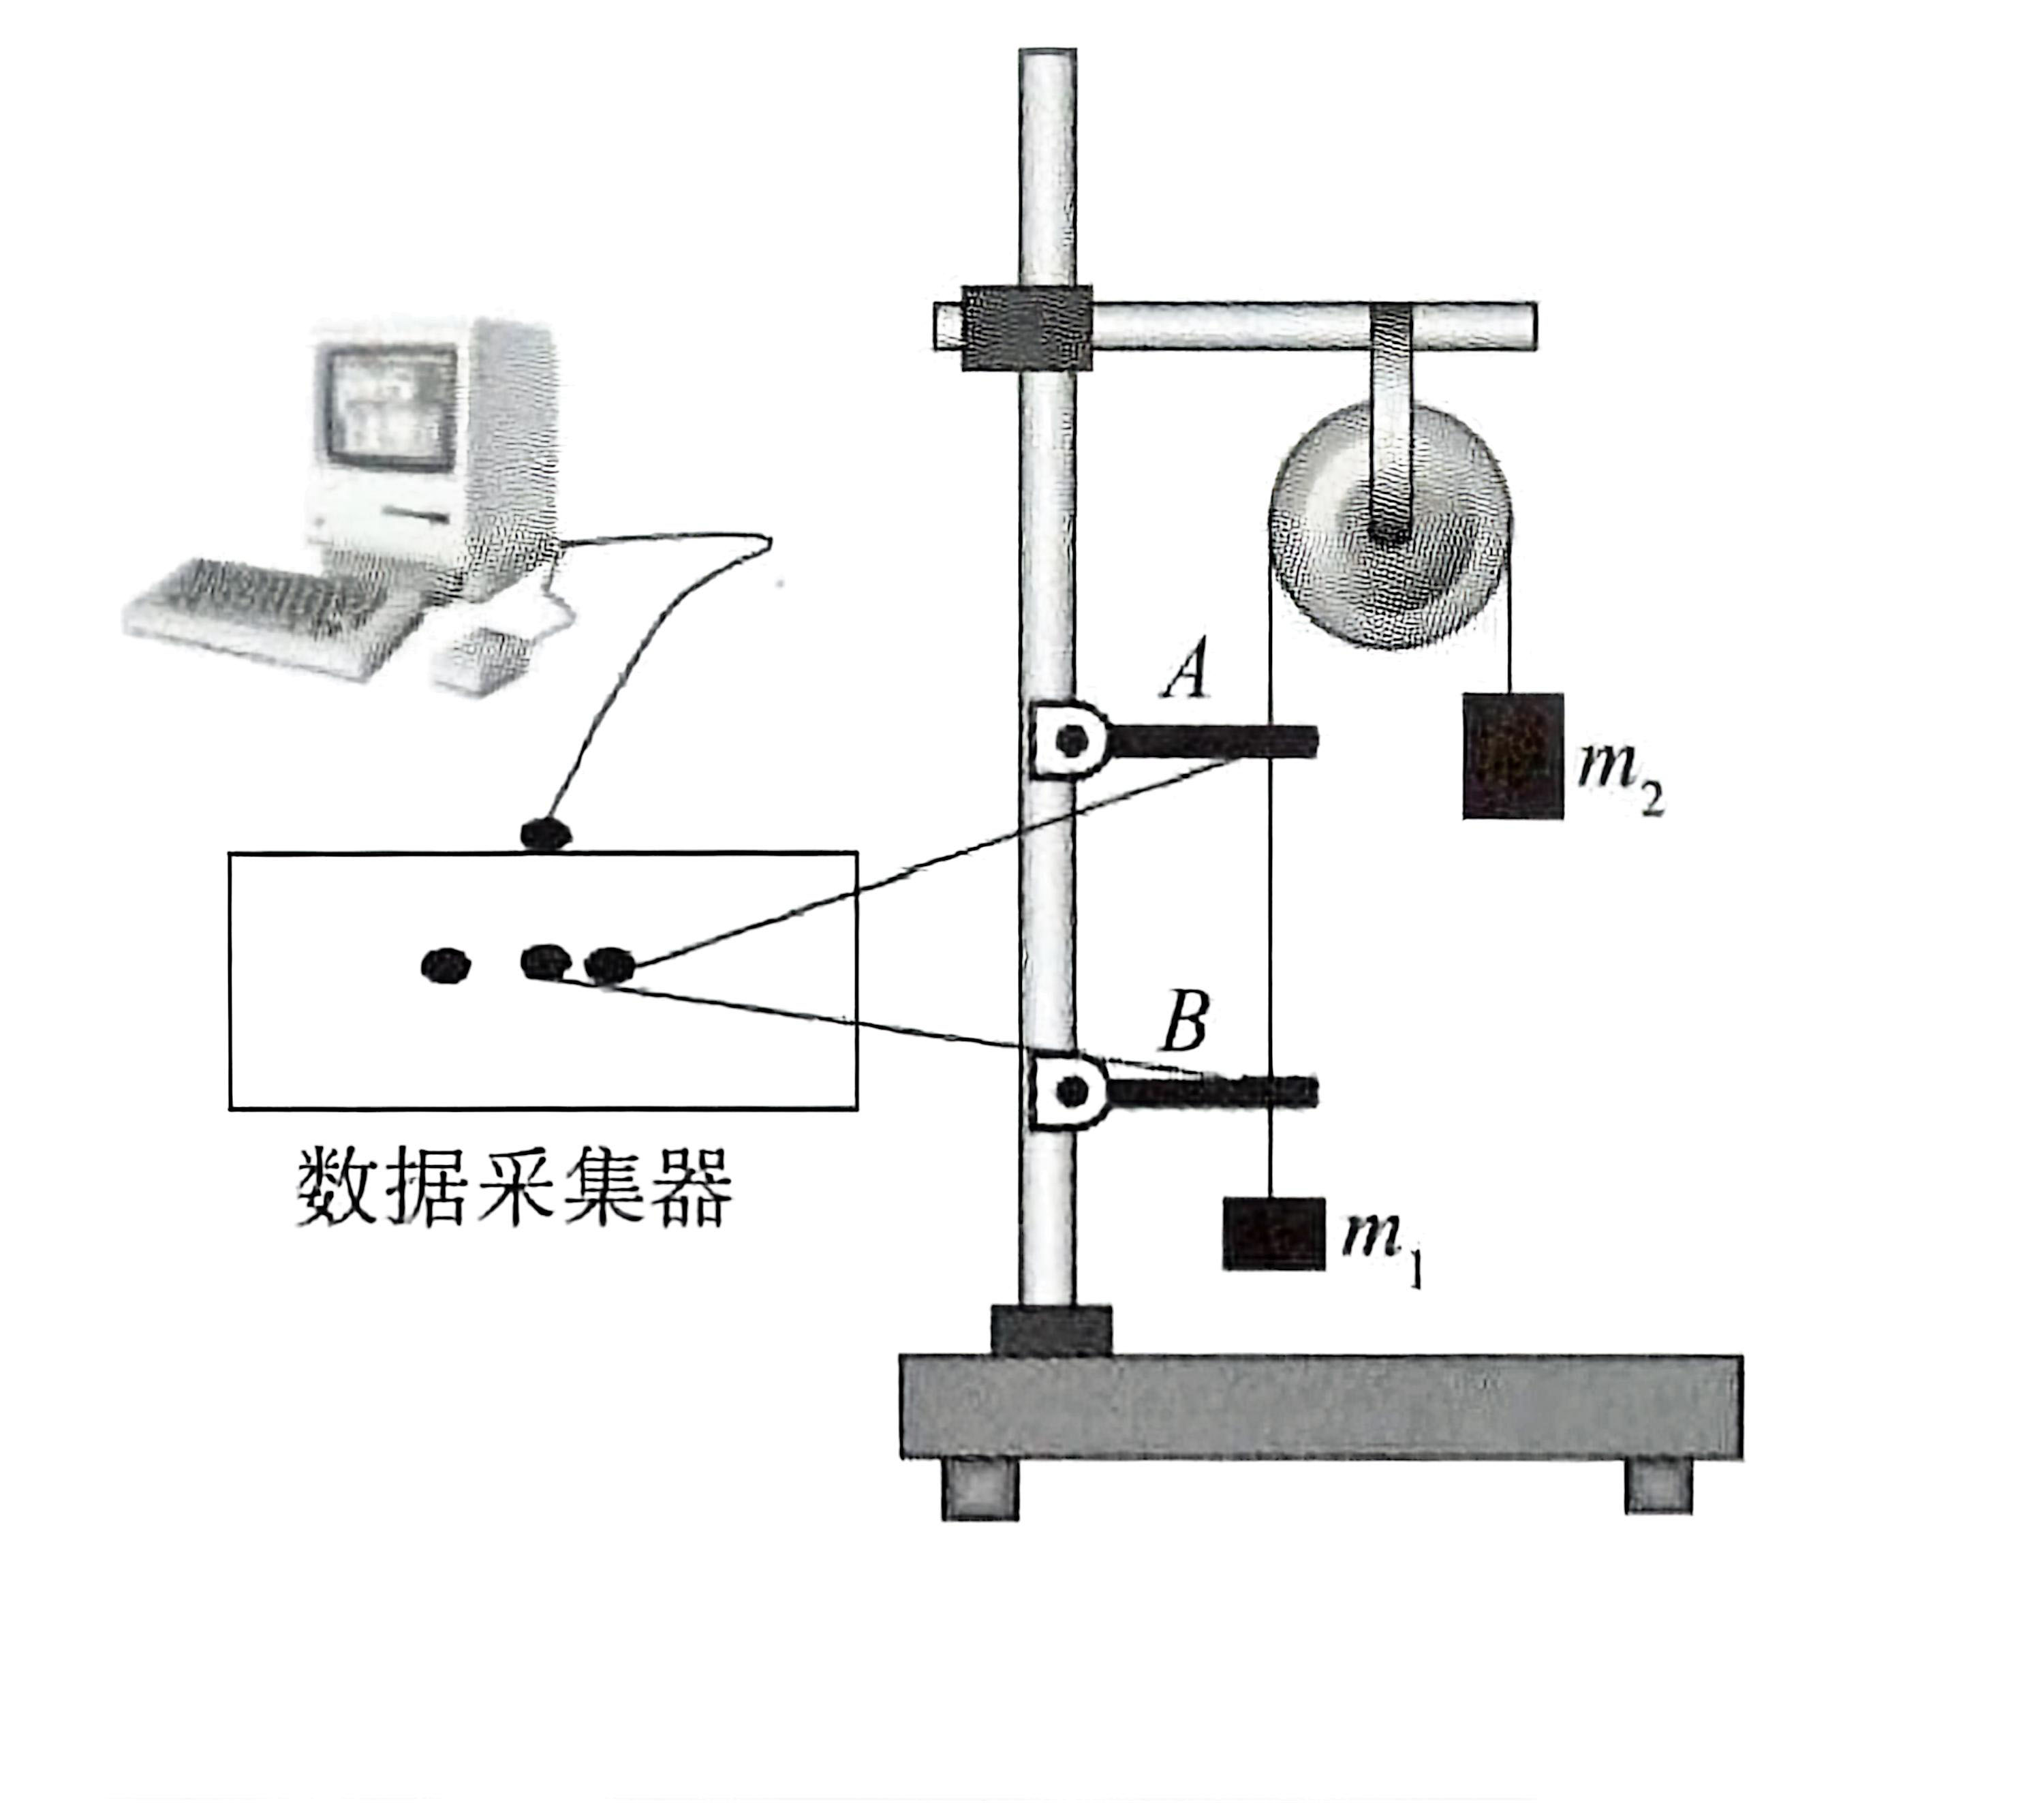
\includegraphics[width=0.4\textwidth]{figures/阿特伍德机示意图.jpg}
        \label{fig:atwood_machine}
    }
    \subfigure[Tracker软件界面]{
        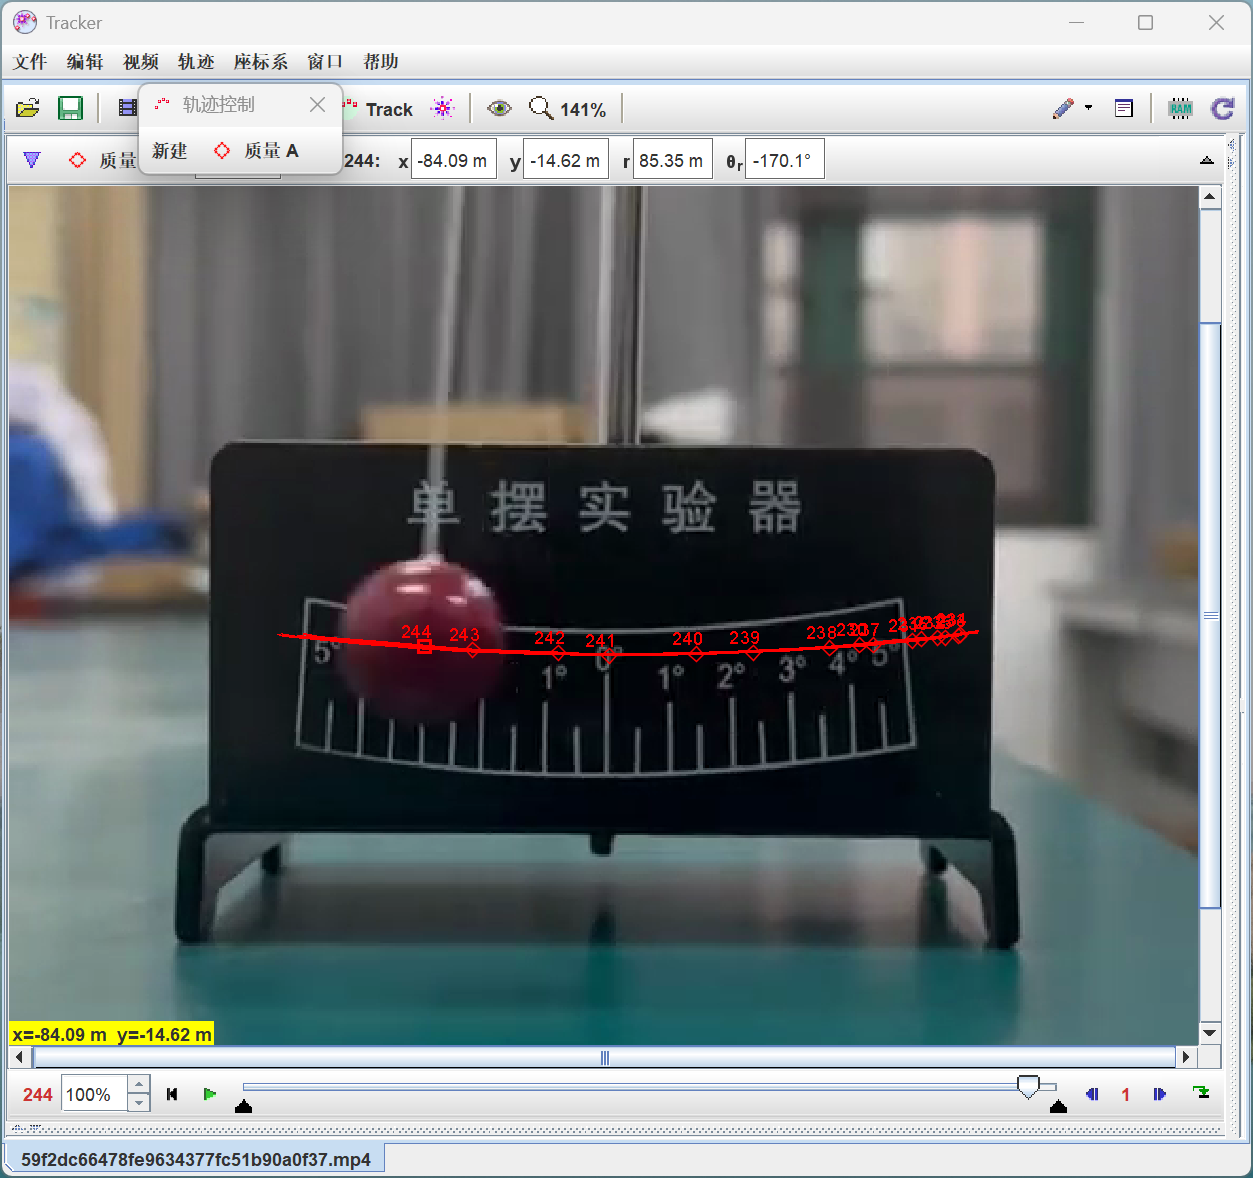
\includegraphics[width=0.4\textwidth]{figures/tracker软件界面.jpg}
        \label{fig:tracker_interface}
    }
    \caption{传统重力加速度测量与分析工具}
    \label{fig:traditional_tools}
\end{figure}


洪炎红等人的研究\textsuperscript{\cite{WLTB201706010}}采用Tracker软件进行重力加速度测量,是一种利用传统计算机视觉技术测量重力加速度的新方法。Tracker是一个基于开源物理(OSP)Java框架的免费视频分析和建模工具\textsuperscript{\cite{brown2009innovative}}。
与Tracker相比,本实验采用的AI辅助系统具有显著优势。本项目采用3502号实验视频,使用本AI辅助系统与Tracker软件分别进行轨迹追踪,将得到的数据文件进行相同的数据处理,对比数据如下:

\begin{table}[H]
\centering
\caption{本系统与Tracker软件对比}
\begin{tabular*}{0.75\textwidth}{@{\extracolsep{\fill}} c c c @{}}
\toprule
\textbf{性能指标} & \textbf{AI辅助系统} & \textbf{Tracker软件} \\
\midrule
识别数据点数 & 631 & 255 \\
测得周期 & 1.189 s & 1.193 s \\
测量精度 & 相对误差为0.12\% & 相对误差为0.85\% \\
背景要求 & 无特殊要求,适应复杂背景 & 需要高对比度,避免杂乱背景 \\
标记要求 & 无需特殊标记物 & 通常需要高对比度标记点 \\
自动化程度 & 全自动跟踪与分析 & 需要手动辅助标记与跟踪 \\
\bottomrule
\end{tabular*}
\label{tab:tracker_comparison}
\end{table}

可见,本系统基于深度学习目标检测算法,能够在无需特殊背景和标记物的情况下精确跟踪运动物体,而Tracker软件通常需要人工设置跟踪点且对背景环境有较高要求。本系统识别目标更加准确,获得了更多的数据点,这为获取高精度实验数据提供了坚实基础,最终的相对误差也显著降低。

\begin{SecondaryBox}[重力加速度测量结果 ]
通过5组数据的综合分析,最终测得的重力加速度平均值为$g = 9.785$ m/s$^2$,与武汉地区标准值$9.7936$ m/s$^2$相比,最佳测量结果的相对误差仅为0.02\%,平均相对误差为0.19\%。测量精度显著优于传统的测量方法,充分证明了AI辅助测量系统的高精度性能。
\end{SecondaryBox}

\subsubsection{周期计算方法对比}

本系统创新性地应用三种互补的周期计算方法,充分利用\textbf{AI赋能的数据收集优势},大幅提高测量精度。以下为摆长0.3501 m、5°初始角度条件下的对比数据:

\begin{table}[H]
\centering
\caption{不同周期计算方法的结果对比(来自3502\_trajectory\_data\_analysis.txt数据)}
\begin{tabular*}{0.9\textwidth}{@{\extracolsep{\fill}} c c c c c@{}}
\toprule
\textbf{计算方法} & \textbf{测量周期(s)} & \textbf{标准差} & \textbf{重力加速度(m/s$^2$)} & \textbf{相对误差(\%)} \\
\midrule
FFT频谱分析法 & 1.189 & - & 9.781 & 0.12 \\
峰值检测法 & 1.192 & 0.007 & 9.740 & 0.55 \\
曲线拟合法 & 1.193 & - & 9.719 & 0.77 \\
最优结果(FFT) & 1.189 & - & 9.781 & 0.12 \\
\bottomrule
\end{tabular*}
\label{tab:period_methods}
\end{table}

如表\ref{tab:period_methods}所示,各种方法测量结果较为接近,但FFT频谱分析法在本例中精度最高。系统默认采用相对误差最小的结果作为最终值。三种方法的特点比较:

\begin{enumerate}[leftmargin=*]
    \item 快速傅里叶变换法:将时域信号转换至频域,通过能量分布识别主频率。本系统采用Hanning窗函数预处理与零填充技术增强频率分辨率,优势是噪声抑制能力强,在5个测量数据中有3次被选为最优方法。在数据3502中表现最佳,相对误差仅为0.12\%;
    
    \item 峰值检测法:直接在时域识别相邻波峰之间的时间差,计算最直观且高效,对于信噪比较高的场景表现良好,但对噪声较敏感。在5个测量数据中有1次被选为最优方法,在数据3504中表现最佳,相对误差为0.11\%;
    
    \item 曲线拟合法:基于物理模型$x(t) = A\sin(\omega t + \phi) + C$,通过非线性最小二乘法拟合,利用全部数据点信息,抗噪性能良好,但拟合结果对初始值敏感,可能存在拟合失败的情况。
\end{enumerate}

\begin{figure}[ht]
    \centering
    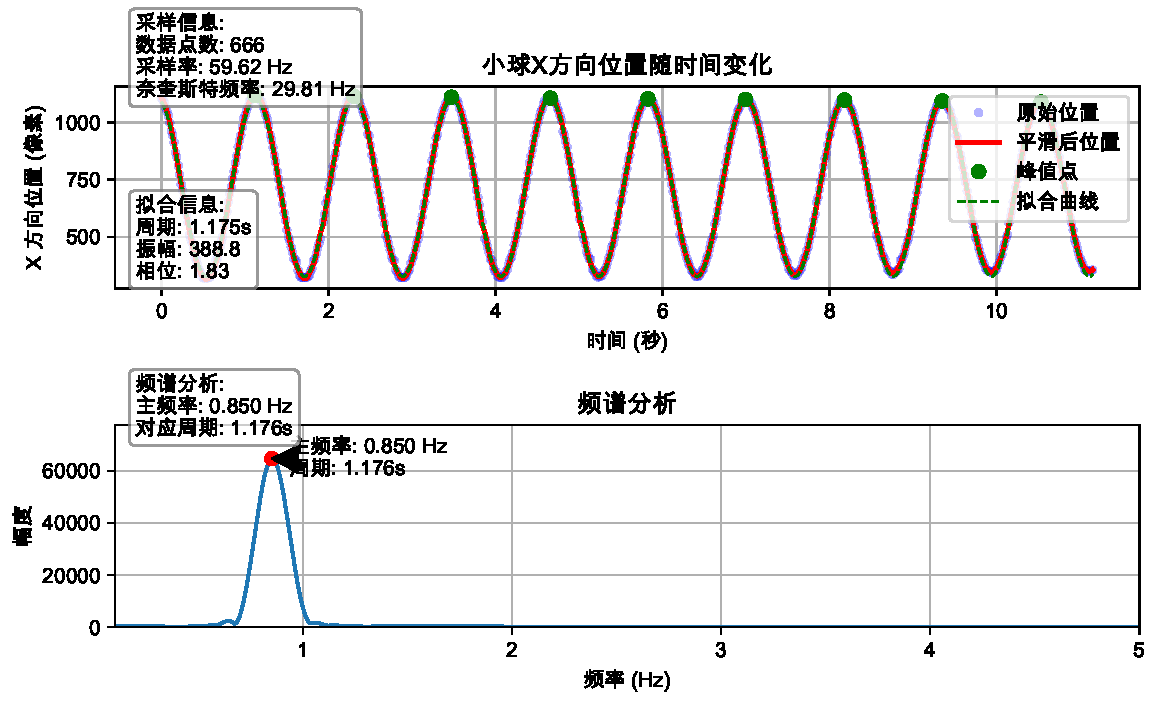
\includegraphics[width=0.7\textwidth]{figures/重力加速度分析结果可视化.pdf}
    \caption{重力加速度测量的波形分析与频谱分析图}
    \label{fig:gravity_analysis}
\end{figure}

如图\ref{fig:gravity_analysis}所示,系统生成的分析图直观显示了平滑后的位置-时间曲线与拟合结果,同时提供频谱分析结果用于验证。观察图中上部可见系统还标记了峰值点位置,用于峰值检测法计算,下部的频谱分析清晰标示出主频率位置。

\subsubsection{摆长与周期的关系分析}

为验证单摆周期公式$T = 2\pi\sqrt{l/g}$,实验采用五组不同摆长(0.33 m-0.37 m)进行测量,通过\textbf{AI视觉跟踪系统获取高精度位置数据},使用多种方法分析周期。实验结果如下:

\begin{table}[H]
\centering
\caption{不同摆长的周期与重力加速度测量结果}
\begin{tabular}{@{}c c c c c@{}}
\toprule
\textbf{摆长(m)} & \textbf{最终周期(s)} & \textbf{采用方法} & \textbf{重力加速度(m/s$^2$)} & \textbf{误差(\%)} \\
\midrule
0.33 & 1.155 & Peak & 9.774 & 0.2 \\
0.34 & 1.174 & FFT & 9.747 & 0.47 \\
0.35 & 1.193 & Fit & 9.725 & 0.7 \\
0.36 & 1.210 & Peak & 9.725 & 0.7 \\
0.37 & 1.225 & FFT & 9.765 & 0.29 \\
\bottomrule
\end{tabular}
\label{tab:lengths_periods}
\end{table}

如表\ref{tab:lengths_periods}所示,对于每个摆长,系统分别使用傅里叶变换法(FFT)、峰值检测法(Peak)和曲线拟合法(Fit)三种方法计算周期,并根据相对误差自动选择最优方法作为最终结果。

将周期$T$对摆长平方根$\sqrt{l}$作图,如图\ref{fig:period_length}所示,呈现出良好的线性关系,符合理论预期。
实验数据点与拟合直线高度吻合,得到拟合方程$T = 2.0463 \cdot \sqrt{l} - 0.0190$,
决定系数$R^2 = 0.9995$,表明线性拟合程度极佳。

\begin{figure}[H]
    \centering
    \begin{tikzpicture}[scale=0.8]
    % 设置坐标系
    \begin{axis}[
        width=0.85\textwidth,
        height=0.6\textwidth,
        xlabel={摆长平方根 $\sqrt{l}$ (m$^{1/2}$)},
        ylabel={周期 $T$ (s)},
        xlabel style={font=\small},
        ylabel style={font=\small},
        xmin=0.565, xmax=0.615,
        ymin=1.14, ymax=1.24,
        tick align=inside,
        xtick={0.57, 0.58, 0.59, 0.60, 0.61},
        ytick={1.15, 1.17, 1.19, 1.21, 1.23},
        ymajorgrids=true,
        xmajorgrids=true,
        grid style={gray!30, solid, line width=0.5pt},
        legend style={at={(0.05,0.95)}, anchor=north west, font=\small, draw},
        tick label style={font=\small},
        title style={font=\bfseries\small}
    ]
    
    % 绘制数据点(带误差棒)
    \addplot[only marks, mark=*, mark size=3pt, mark options={fill=blue}, error bars/.cd, y dir=both, y explicit, 
    error bar style={line width=0.8pt, color=black}, error mark options={line width=0.8pt, mark size=3pt, rotate=90}] 
    coordinates {
        (0.5745, 1.155) +- (0, 0.0012)  % sqrt(0.33)
        (0.5831, 1.174) +- (0, 0.0028)  % sqrt(0.34)
        (0.5916, 1.193) +- (0, 0.0042)  % sqrt(0.35)
        (0.6000, 1.210) +- (0, 0.0042)  % sqrt(0.36)
        (0.6083, 1.225) +- (0, 0.0018)  % sqrt(0.37)
    };
    
    % 绘制拟合线
    \addplot[orange, dashed, line width=1.5pt, domain=0.565:0.615] {2.0463*x - 0.0190};
    
    % 添加图例
    \legend{实验数据, {理论拟合: $T = 2.0463 \cdot \sqrt{l} - 0.0190$,$R^2 = 0.9995$}};
    
    \end{axis}
\end{tikzpicture}
    \caption{周期与摆长平方根的线性关系图}
    \label{fig:period_length}
\end{figure}

\begin{SecondaryBox}[周期与摆长平方根的线性关系]
\quad \quad 从拟合结果可知,斜率$k = 2.0463$,代入$k = 2\pi/\sqrt{g}$,可以反算得到$g = 4\pi^2/k^2 = 9.779$ m/s$^2$。
这一结果与武汉地区标准重力加速度值$9.7936$ m/s$^2$非常接近,相对误差仅为0.15\%。
拟合直线的截距为$-0.0190$,理论上应为零,这一微小偏差可能来源于测量系统的系统误差或摆长测量的零点误差。
\end{SecondaryBox}





\subsubsection{大摆角下非线性修正效果}

大摆角条件下,单摆运动不再满足小角度近似,周期会随振幅增大而增加。系统通过非线性周期修正处理该问题:

\begin{equation}
T = T_0 \cdot (1 + \frac{1}{16}\theta^2 + \frac{11}{3072}\theta^4 + ...)
\end{equation}

其中$T_0$为小摆角条件下的理论周期,$\theta$为弧度制的初始摆角。实验通过一系列不同摆角验证该修正有效性:

\begin{table}[H]
\centering
\caption{不同初始摆角的周期与重力加速度测量结果(摆长0.35 m)}
\begin{tabular}{@{}cccccc@{}}
\toprule
\textbf{初始摆角(°)} & \textbf{未修正g值(m/s$^2$)} & \textbf{未修正误差(\%)} & \textbf{修正系数} & \textbf{修正后g值(m/s$^2$)} & \textbf{修正后误差(\%)} \\
\midrule
5 & 9.716 & 0.79 & 1.000476 & 9.725 & 0.70 \\
10 & 9.758 & 0.36 & 1.001907 & 9.795 & 0.02 \\
15 & 9.751 & 0.43 & 1.004301 & 9.835 & 0.43 \\
20 & 9.679 & 1.17 & 1.007669 & 9.828 & 0.35 \\
25 & 9.604 & 1.93 & 1.012029 & 9.837 & 0.44 \\
\bottomrule
\end{tabular}
\label{tab:angle_periods}
\end{table}

数据表明,\textbf{随着摆角增大,非线性效应逐渐显著}。

\begin{SecondaryBox}[大摆角修正效果分析]
分析表\ref{tab:angle_periods}数据可以发现:

1. 修正系数随摆角增大而增加,从5°时的1.000476增至25°时的1.012029,表明大摆角下非线性效应显著增强。

2. 摆角为5°时,未修正重力加速度值为9.716 m/s²,相对误差为0.79\%;当摆角增至25°时,未修正值下降至9.604 m/s²,相对误差增至1.93\%,可见摆角对测量结果的显著影响。

3. 应用非线性修正后,即使在25°的大摆角下,相对误差也能控制在0.44\%以内,而10°条件下的修正效果最佳,相对误差仅为0.02\%,这表明非线性修正显著提高了大摆角条件下的测量精度。

4. 通过对比三种测量方法(FFT、Peak和Fit),系统能够根据不同摆角条件自动选择最优测量方法,5°和25°时选择Fit方法,10°时选择FFT方法,15°和20°时选择Peak方法,这种智能选择进一步优化了测量结果。
\end{SecondaryBox}

\subsection{阻尼系数测量的数据分析}


\subsubsection{阻尼系数测量的测量结果}
本实验利用AI视觉追踪系统,对摆长为0.8 m、摆球质量为0.004 kg的单摆进行了5次重复阻尼特性测量,获得了高精度的阻尼参数数据。测量结果汇总如下表所示:

\begin{table}[H]
\centering
\caption{摆长为0.8 m的单摆阻尼测量结果}
\begin{tabular}{@{}c c c c c c c@{}}
\toprule
\textbf{编号} & \textbf{初始振幅} & \textbf{$n$周期后振幅} & \textbf{周期数$n$} & \textbf{周期$T$(s)} & \textbf{阻尼系数$\beta$(N·s/m)} & \textbf{时间常数$\tau$(s)} \\
\midrule
1 & 349.46 & 115.53 & 33 & 1.788 & 0.000075 & 53.30 \\
2 & 344.50 & 114.35 & 33 & 1.788 & 0.000075 & 53.49 \\
3 & 347.64 & 115.01 & 33 & 1.789 & 0.000075 & 53.37 \\
4 & 345.50 & 113.87 & 33 & 1.787 & 0.000075 & 53.13 \\
5 & 349.34 & 112.48 & 33 & 1.788 & 0.000077 & 52.06 \\
\textbf{平均值} & 347.29 & 114.25 & - & 1.788 & 0.000075 & 53.07 \\
\textbf{标准差} & 2.22 & 1.16 & - & 0.001 & 0.000001 & 0.57 \\
\bottomrule
\end{tabular}
\label{tab:damping_results}
\end{table}

\begin{SecondaryBox}[阻尼系数测量结果]
从表\ref{tab:damping_results}中可以看出,5次测量结果具有良好的一致性,阻尼系数$\beta$的平均值为0.000075 N·s/m,与同类实验结果相接近。
衰减时间常数$\tau$平均为53.07 s,意味着振幅需要约0.88 min才能衰减至初始值的36.8\%(即$1/e$倍),表明该单摆系统阻尼较小,属于典型的弱阻尼系统。
数据的标准差较小,证明了实验测量的重复性和可靠性,同时也表明AI视觉跟踪系统能够稳定地测量阻尼振动过程。
\end{SecondaryBox}



\subsubsection{阻尼特性量化与参数分析}

系统通过自动追踪摆球位置,提取振幅随时间变化的完整数据,应用指数衰减模型 $A(t) = A_0e^{-\frac{\beta}{m} t}$精确量化阻尼特性,
与传统人工测量相比,系统测量阻尼特性参数的优势体现在:
\begin{enumerate}[leftmargin=*]
    \item 高密度数据采集:传统方法通常仅测量有限几个振幅值点,而本系统可提取视频中每一帧的位置数据,获得连续的阻尼衰减过程;
    
    \item 自动峰值识别:系统自动识别所有波峰并提取振幅值,消除了人工计时与目测误差;
    
    \item 对数衰减法:系统自动计算振幅的对数值并进行线性拟合,从斜率直接获得阻尼系数与质量比值$\beta/m$的相反数,大幅提高量化精度。
\end{enumerate}

如图\ref{fig:damping_analysis}所示,上图展示小球位置随时间变化的阻尼振动曲线及其拟合曲线,下图为振幅对数值随时间变化的线性关系图。对数图的斜率即为阻尼系数的负值,实现了直观的阻尼效应量化。


\begin{figure}[H]
    \centering
    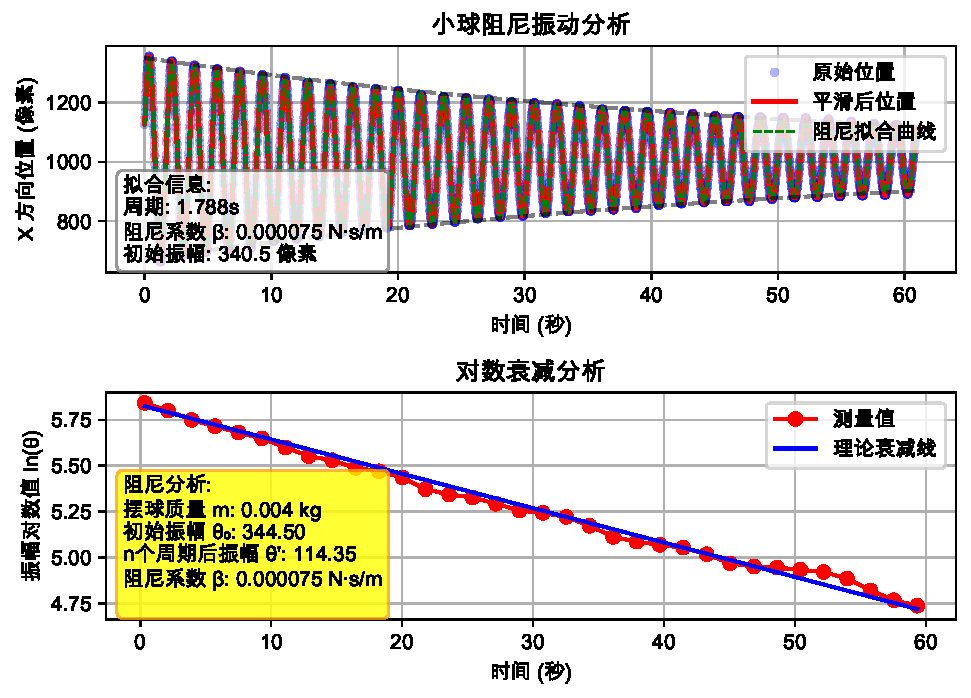
\includegraphics[width=0.65\textwidth]{figures/22_trajectory_data_damping_analysis.pdf}
    \caption{阻尼振动分析与对数衰减图}
    \label{fig:damping_analysis}
\end{figure}



实验在摆长0.8 m条件下进行,获得完整的阻尼参数集,如表\ref{tab:damping_params}所示,

\begin{table}[H]
\centering
\caption{阻尼振动的关键参数测量结果}
\setlength{\tabcolsep}{7mm}
\begin{tabular}[c]{c c c c}
\toprule
{\textbf{参数}} & {\textbf{测量值}} & {\textbf{单位}} \\
\midrule
阻尼系数 $\beta$ & 0.000075 & N$\cdot$s/m \\
固有角频率 $\omega_0$ & 3.5144 & rad/s \\
振动周期 $T$ & 1.788 & s \\
品质因数 $Q$ & 93.26 & 无量纲 \\
衰减时间常数 $\tau$ & 53.07 & s \\
\bottomrule
\end{tabular}
\label{tab:damping_params}
\end{table}

其中品质因数Q\textsuperscript{\cite{DXWL201705004}}:定义为$Q = \frac{m\omega_0}{\beta}$,表征系统振动能量的存储能力,Q值越大表示系统阻尼越小,能量损失率越低。测得Q = 93.26表明该系统属于低阻尼类型;衰减时间常数τ:定义为$\tau = m/\beta$,表示振幅衰减至初始值的1/e所需时间,是量化振动持续时间的重要指标。测得τ = 53.07 s说明该单摆系统能够保持较长时间的振动状态,这两个指标排除出了质量的影响,为探究阻尼特性影响因素提供了参考指标。


\subsubsection{阻尼特性影响因素分析}

为探究影响单摆阻尼特性的主要因素,本团队设计了一系列对比实验,系统分析了摆长、摆球尺寸和摆球质量三个关键因素对阻尼特性的影响。下面将分别详细讨论各因素对阻尼系数($\beta$)、衰减系数($\gamma$)、衰减时间常数($\tau$)、品质因数($Q$)等阻尼特性参数的综合影响。

\textbf{1)摆长对阻尼特性的影响},为探究摆长对阻尼特性的影响,本团队使用固定质量(0.009 kg)的塑料大球,在5°初始摆角条件下,进行了一系列不同摆长(0.4 m至1.0 m)的阻尼特性对比实验。实验结果如表\ref{tab:length_damping}所示。

\begin{table}[H]
\centering
\caption{摆长对阻尼特性的影响}
\begin{tabular}{c c c c c c@{}}
\toprule
\textbf{摆长(m)} & \textbf{周期(s)} & \textbf{阻尼系数$\beta$(N$\cdot$s/m)} & \textbf{衰减系数$\gamma$(s$^{-1}$)} & \textbf{品质因数$Q$} & \textbf{衰减时间常数$\tau$(s)} \\
\midrule
0.40 & 1.278 & 0.000091 & 0.010147 & 484.46 & 98.55 \\
0.55 & 1.496 & 0.000102 & 0.011336 & 370.46 & 88.21 \\
0.70 & 1.683 & 0.000104 & 0.011606 & 321.60 & 86.16 \\
0.85 & 1.855 & 0.000108 & 0.011979 & 282.76 & 83.48 \\
1.00 & 2.004 & 0.000118 & 0.013151 & 238.38 & 76.04 \\
\bottomrule
\end{tabular}
\label{tab:length_damping}
\end{table}

实验数据显示,随着摆长从0.4 m增加到1.0 m:
\begin{itemize}
  \item 振动周期T随摆长增加而显著增加,从1.278 s增至2.004 s,增幅约57\%,符合理论预期$T = 2\pi\sqrt{l/g}$;
  \item 阻尼系数$\beta$随摆长增加而增大约30\%(从0.000091增至0.000118 N·s/m);
  \item 衰减系数$\gamma$(单位质量的阻尼系数)增加约30\%(从0.010147增至0.013151 s$^{-1}$);
  \item 品质因数$Q$显著降低约51\%(从484.46降至238.38);
  \item 衰减时间常数$\tau$降低约23\%(从98.55降至76.04 s);
\end{itemize}

这种变化趋势表明,摆长对单摆系统的阻尼特性有显著影响。摆长增加导致摆球的线速度提高,增加了与空气的相对运动速度,从而增大了空气阻力,表现为阻尼系数的增加。此外,摆长增加改变了整个系统的运动特性,使得能量损耗相对增加,表现为品质因数的降低和衰减时间常数的减小。

\begin{figure}[H]
    \centering
    \subfigure[摆长对阻尼系数的影响]{
        \begin{tikzpicture}[scale=0.5]
    % 设置坐标系
    \begin{axis}[
        width=0.85\textwidth,
        height=0.6\textwidth,
        xlabel={摆长 $l$ (m)},
        ylabel={阻尼系数 $\beta$ (N$\cdot$s/m)},
        xlabel style={font=\small},
        ylabel style={font=\small},
        xmin=0.35, xmax=1.05,
        ymin=0.00008, ymax=0.00012,
        tick align=inside,
        xtick={0.4, 0.55, 0.7, 0.85, 1.0},
        ytick={0.00009, 0.000095, 0.0001, 0.000105, 0.00011, 0.000115, 0.00012},
        yticklabel style={/pgf/number format/fixed, /pgf/number format/precision=6},
        ymajorgrids=true,
        xmajorgrids=true,
        grid style={gray!30, solid, line width=0.5pt},
        legend style={at={(0.05,0.95)}, anchor=north west, font=\small, draw},
        tick label style={font=\small},
        title style={font=\bfseries\small}
    ]
    
    % 绘制数据点
    \addplot[only marks, mark=*, mark size=3pt, mark options={fill=blue}] 
    coordinates {
        (0.40, 0.000091)
        (0.55, 0.000102)
        (0.70, 0.000104)
        (0.85, 0.000108)
        (1.00, 0.000118)
    };
    
    % 绘制拟合线
    \addplot[orange, dashed, line width=1.5pt, domain=0.35:1.05] {0.00004*x + 0.0000766};
    
    % 添加图例
    \legend{实验数据, {线性拟合: $\beta = 4.00 \times 10^{-5} \cdot l + 7.66 \times 10^{-5}$, $R^2 = 0.9395$}};
    
    \end{axis}
\end{tikzpicture}
        \label{fig:length_damping_coef}
    }
    \subfigure[摆长对品质因数的影响]{
        \begin{tikzpicture}[scale=0.5]
    % 设置坐标系
    \begin{axis}[
        width=0.85\textwidth,
        height=0.6\textwidth,
        xlabel={摆长 $l$ (m)},
        ylabel={品质因数 $Q$},
        xlabel style={font=\small},
        ylabel style={font=\small},
        xmin=0.35, xmax=1.05,
        ymin=220, ymax=500,
        tick align=inside,
        xtick={0.4, 0.55, 0.7, 0.85, 1.0},
        ytick={220, 270, 320, 370, 420, 470},
        ymajorgrids=true,
        xmajorgrids=true,
        grid style={gray!30, solid, line width=0.5pt},
        legend style={at={(0.95,0.95)}, anchor=north east, font=\small, draw},
        tick label style={font=\small},
        title style={font=\bfseries\small}
    ]
    
    % 绘制数据点
    \addplot[only marks, mark=*, mark size=3pt, mark options={fill=blue}] 
    coordinates {
        (0.40, 484.46)
        (0.55, 370.46)
        (0.70, 321.60)
        (0.85, 282.76)
        (1.00, 238.38)
    };
    
    % 绘制二次拟合线 (使用MATLAB代码中计算的系数)
    \addplot[orange, dashed, line width=1.5pt, domain=0.35:1.05] {473.84*x^2 - 1049.95*x + 820.99};
    
    % 添加图例
    \legend{实验数据, {二次拟合: $Q = 473.84 l^2 - 1049.95 l + 820.99$, $R^2 = 0.9854$}};
    
    \end{axis}
\end{tikzpicture}
        \label{fig:length_quality_factor}
    }
    \caption{摆长对阻尼系数和品质因数的影响}
    \label{fig:length_damping}
\end{figure}

如图\ref{fig:length_damping}所示,阻尼系数$\beta$与摆长呈增长关系,而品质因数$Q$则随摆长增加而显著下降。

\textbf{2)摆球尺寸对阻尼特性的影响},为探究摆球尺寸对阻尼特性的影响,本团队使用两种不同直径的塑料球进行对比实验,并保持摆长(0.8m)不变,为排除质量的影响,本团队主要分析衰减系数$\gamma$、品质因数$Q$和衰减时间常数$\tau$。实验结果如表\ref{tab:size_damping}所示。

\begin{table}[H]
\centering
\caption{摆球尺寸对阻尼特性的影响}
\begin{tabular}{c c c c c c@{}}
\toprule
\textbf{球类型} & \textbf{质量(kg)} & \textbf{阻尼系数$\beta$(N$\cdot$s/m)} & \textbf{衰减系数$\gamma$(s$^{-1}$)} & \textbf{品质因数$Q$} & \textbf{衰减时间常数$\tau$(s)} \\
\midrule
塑料小球 & 0.004 & 0.000089 & 0.022295 & 157.90 & 44.86 \\
塑料大球 & 0.009 & 0.000104 & 0.011508 & 307.46 & 86.98 \\
\bottomrule
\end{tabular}
\label{tab:size_damping}
\end{table}

实验数据显示,随着球体尺寸增大(质量从0.004 kg增至0.009 kg):
\begin{itemize}
  \item 衰减系数$\gamma$(单位质量的阻尼系数)降低约48\%(从0.022295降至0.011508 s$^{-1}$);
  \item 品质因数$Q$提高约95\%(从157.90增至307.46);
  \item 衰减时间常数$\tau$提高约94\%(从44.86增至86.98 s);
\end{itemize}

\textbf{3)摆球质量对阻尼特性的影响},为研究质量对阻尼特性的影响,本团队比较了两种不同质量的相同尺寸摆球:不锈钢小球(0.031 kg)和塑料小球(0.004 kg),实验过程中保持摆长(0.8 m)和初始角度(5°)不变。实验结果如表\ref{tab:material_damping}所示。

\begin{table}[H]
\centering
\caption{摆球质量对阻尼特性的影响}
\begin{tabular}{@{}c c c c c c@{}}
\toprule
\textbf{摆球类型} & \textbf{质量(kg)} & \textbf{阻尼系数$\beta$(N$\cdot$s/m)} & \textbf{衰减系数$\gamma$(s$^{-1}$)} & \textbf{品质因数$Q$} & \textbf{衰减时间常数$\tau$(s)} \\
\midrule
不锈钢小球 & 0.031 & 0.000115 & 0.0037 & 941.40 & 269.39 \\
塑料小球 & 0.004 & 0.000089 & 0.0223 & 157.90 & 44.86 \\
\bottomrule
\end{tabular}
\label{tab:material_damping}
\end{table}

实验数据表明,在相同摆长和初始角度条件下,两种不同质量的相同尺寸摆球表现出显著不同的阻尼特性:
\begin{itemize}
  \item 阻尼系数$\beta$随质量增大而略微增大(从0.000089增至0.000115 N·s/m),增幅约29\%
  \item 衰减系数$\gamma=\beta/m$随质量增大而显著降低,塑料球(0.0223 s$^{-1}$)约为不锈钢球(0.0037 s$^{-1}$)的6倍
  \item 不锈钢球的品质因数$Q$远高于塑料球,为941.40,是塑料球(157.90)的约6倍
  \item 不锈钢球的衰减时间常数$\tau$显著长于塑料球,达269.39 s,是塑料球(44.86 s)的约6倍
\end{itemize}

通过对摆长、摆球尺寸和摆球质量三个因素的系统研究,得出以下结论:
\begin{SecondaryBox}[阻尼特性影响因素分析]

1. 摆长对阻尼特性的影响:
   实验表明,摆长从0.4 m增加至1.0 m时,阻尼系数$\beta$增大约30\%,品质因数$Q$下降约51\%,衰减时间常数$\tau$减小约23\%。这一现象可归因于摆长增加导致摆球线速度增大,从而增强了与速度相关的空气阻力,加快了系统能量的耗散速率。

2. 摆球尺寸对阻尼特性的影响:
   对于相同材质的摆球,当尺寸增大时,衰减系数$\gamma$降低约48\%,品质因数$Q$和衰减时间常数$\tau$均提高约95\%。这是因为摆球质量(与半径的三次方成正比,$\propto r^3$)增长速率快于其横截面积(与半径的平方成正比,$\propto r^2$),导致单位质量所受阻尼减小,系统惯性增强。

3. 摆球质量对阻尼特性的影响:
   实验数据显示,相同尺寸条件下,不锈钢球的衰减系数$\gamma$仅为塑料球的约1/6,品质因数$Q$和衰减时间常数$\tau$约为塑料球的6倍。这主要是因为在相似的空气阻力作用下,不锈钢球质量(0.031 kg)显著大于塑料球(0.004 kg),使得单位质量的能量损耗率大幅降低。

\quad\quad 综上所述,摆长主要通过改变摆球运动速度影响系统的绝对阻尼大小,而摆球的尺寸和材质则通过改变质量与截面积的比值影响单位质量的阻尼效应。实验结果表明,密度越高、尺寸越大的摆球,其维持振动的能力越强,表现为更高的品质因数和更长的衰减时间常数。
\end{SecondaryBox}